% generated by scripts/pkl_to_latex.py
% source PKL : uscan_v1_L6_Ne6_t1_mode-uniform_nmin2_solver-gcg_sz0_restarts10_iter200_kmax4_tol1em09_U1to20_N20-d03a74da789e.pkl
% scan type  : uscan
% state      : gs
% requires   : \usepackage{pgfplots} \pgfplotsset{compat=1.18}
% colours match the matplotlib PDF (tab10 cycle)
\definecolor{gmeC0}{HTML}{1F77B4}
\definecolor{gmeC1}{HTML}{FF7F0E}
\definecolor{gmeC2}{HTML}{2CA02C}
\definecolor{gmeC3}{HTML}{D62728}
\definecolor{gmeC4}{HTML}{9467BD}
\definecolor{gmeC5}{HTML}{8C564B}
\definecolor{gmeC6}{HTML}{E377C2}
\definecolor{gmeC7}{HTML}{17BECF}

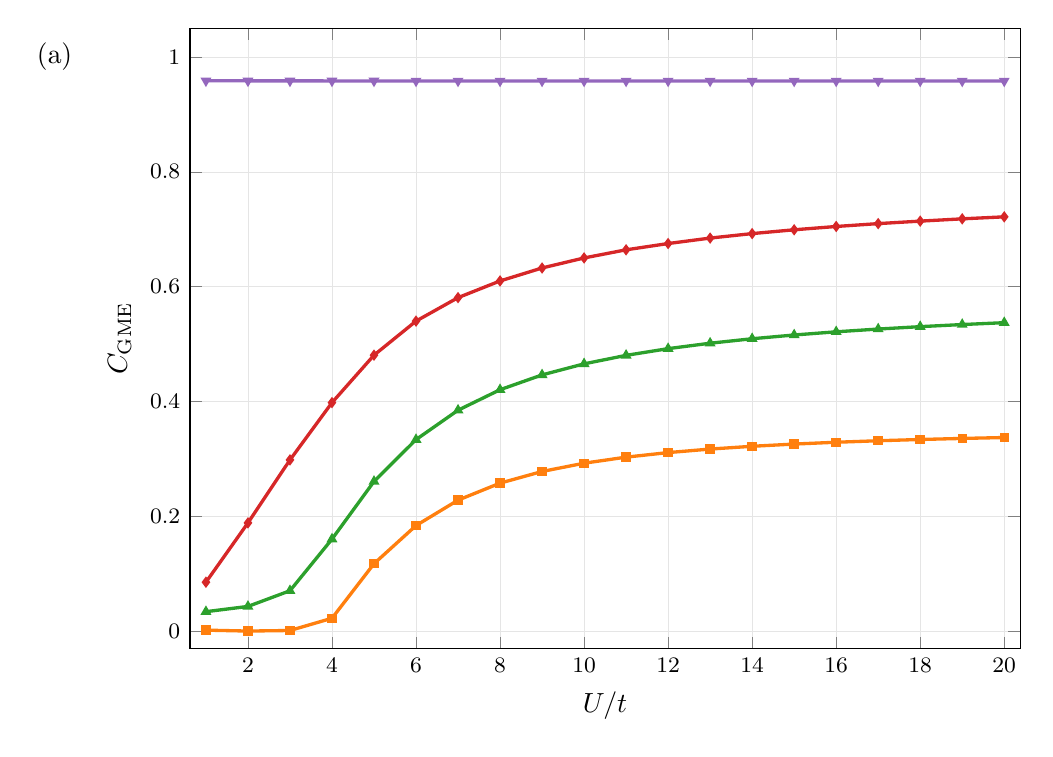
\begin{tikzpicture}
  \begin{axis}[
    width=\columnwidth,
    height=0.78\columnwidth,
    xlabel={$U/t$},
    ylabel={$C_{\mathrm{GME}}$},
    grid=both,
    grid style={line width=.1pt, draw=gray!20},
    tick label style={font=\footnotesize\rmfamily, /pgf/number format/fixed},
    label style={font=\normalsize\rmfamily},
    scaled ticks=false,
    legend style={font=\scriptsize\rmfamily, draw=gray!40, at={(0.5,1.03)}, anchor=south, /tikz/every even column/.append style={column sep=6pt}},
    legend cell align={left},
    legend columns=2,
    ymin=-0.03,
    ymax=1.05,
    xmin=0.62,
    xmax=20.38,
    after end axis/.append code={\node[anchor=east, font=\normalsize\rmfamily] at (axis description cs:-0.13,0.954) {(a)};},
  ]
    \addplot[color=gmeC1, mark=square*, mark size=1.1pt, line width=1.2pt] coordinates {
        (1,0.001781) (2,0.00019) (3,0.001173) (4,0.022499)
        (5,0.117491) (6,0.183917) (7,0.228184) (8,0.25778)
        (9,0.278095) (10,0.292503) (11,0.303051) (12,0.310996)
        (13,0.317128) (14,0.321962) (15,0.325841) (16,0.329003)
        (17,0.331615) (18,0.333798) (19,0.335642) (20,0.337214)
    };
    \addplot[color=gmeC2, mark=triangle*, mark size=1.1pt, line width=1.2pt] coordinates {
        (1,0.033944) (2,0.04309) (3,0.070399) (4,0.160314)
        (5,0.260682) (6,0.333588) (7,0.384779) (8,0.420468)
        (9,0.446274) (10,0.465514) (11,0.480315) (12,0.492004)
        (13,0.501455) (14,0.509252) (15,0.515782) (16,0.521342)
        (17,0.526132) (18,0.530308) (19,0.533977) (20,0.537224)
    };
    \addplot[color=gmeC3, mark=diamond*, mark size=1.1pt, line width=1.2pt] coordinates {
        (1,0.085269) (2,0.188553) (3,0.298219) (4,0.397994)
        (5,0.480619) (6,0.539958) (7,0.580833) (8,0.609883)
        (9,0.632472) (10,0.649929) (11,0.66411) (12,0.675033)
        (13,0.684552) (14,0.692346) (15,0.698997) (16,0.704738)
        (17,0.709743) (18,0.714062) (19,0.718048) (20,0.721531)
    };
    \addplot[color=gmeC4, mark=triangle*, mark size=1.1pt, mark options={rotate=180}, line width=1.2pt] coordinates {
        (1,0.958508) (2,0.958357) (3,0.958276) (4,0.958232)
        (5,0.958209) (6,0.958197) (7,0.95819) (8,0.958186)
        (9,0.958184) (10,0.958182) (11,0.958181) (12,0.958181)
        (13,0.95818) (14,0.95818) (15,0.95818) (16,0.95818)
        (17,0.95818) (18,0.95818) (19,0.958179) (20,0.958179)
    };
  \end{axis}
\end{tikzpicture}
